
This section presents the design exploration of a set of streaming applications being executed on a DMP.
The section describes how changing the thread mapping and core composition affect the benchmarks and what can be learned from this.
In addition, the impact of loop unrolling and how it helps exploit larger fused cores is investigated.


\begin{figure}[t]
    \centering
    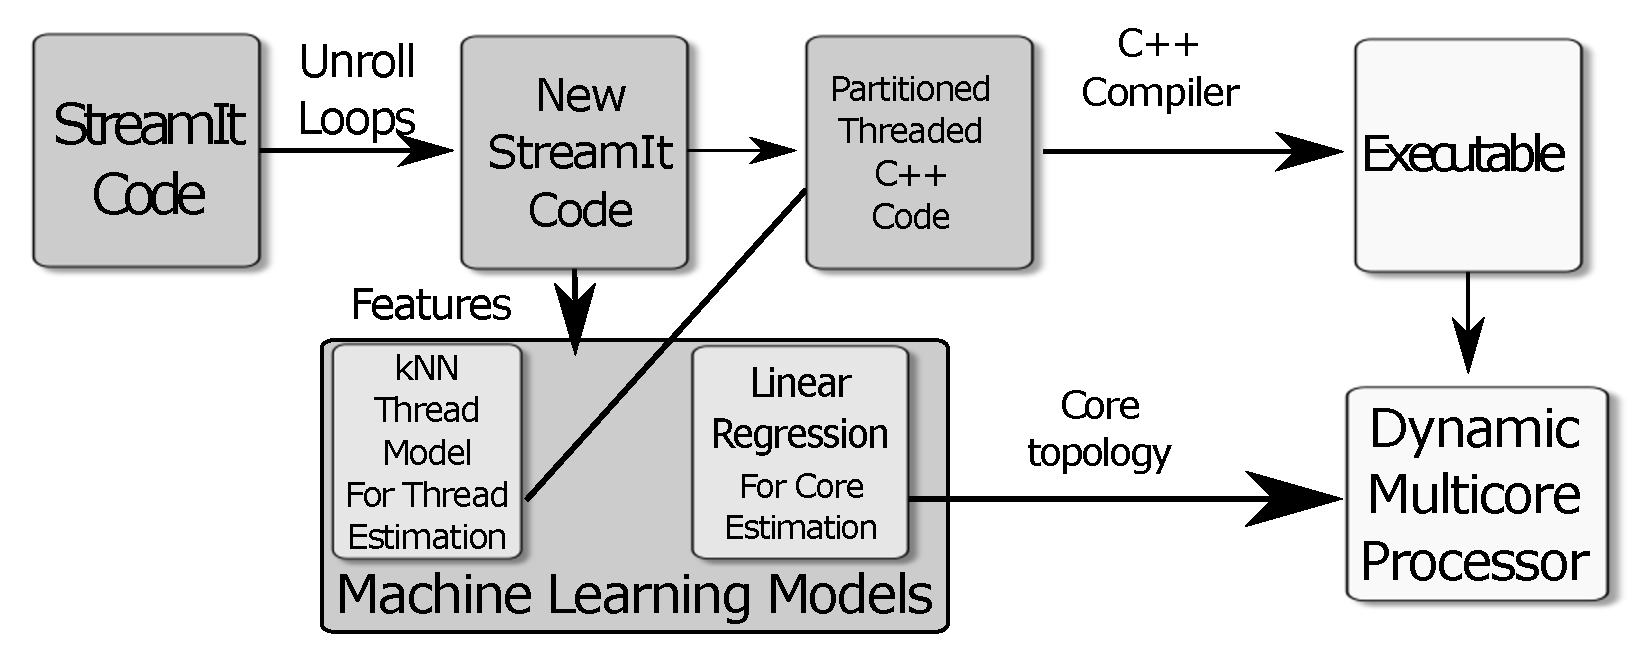
\includegraphics[width=1\textwidth]{streamit-paper/graphics/explanation3.pdf}
    \caption{Description of the workflow.
    Two distinct machine-learning models are used to predict the optimal thread partitioning and core composition based on static code features.}
    \label{fig:overview}
\end{figure}

\subsection{Overview}

\begin{figure}[t]
    \centering
    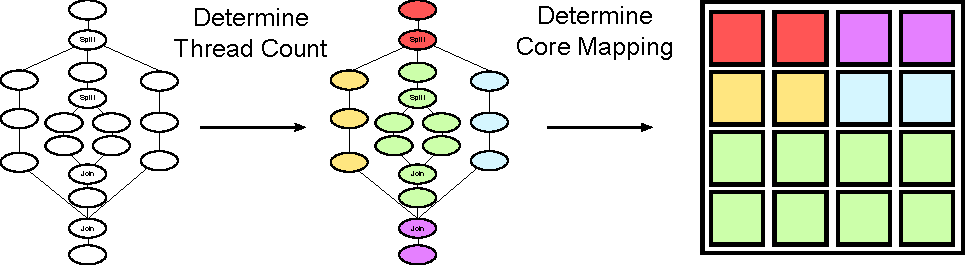
\includegraphics[width=1\textwidth]{streamit-paper/graphics/examplestrem.pdf}
    \caption{Example of a StreamIt program being partitioned into threads (represented by the different colours) followed by assigning cores to each thread.}
    \label{fig:examplestream}
\end{figure}

Figure~\ref{fig:overview} presents the workflow of the system used in this chapter and Figure~\ref{fig:examplestream} illustrates the workflow on a synthetic StreamIt graph.
First, the source-to-source StreamIt compiler is used to unroll loops as this is often beneficial when cores are composed as will be seen later in Section~\ref{sec:streamit:dse}.
Then, static code features such as the program's graph structure are extracted from the StreamIt code through the StreamIt source-to-source compiler.
These features are used as an input to the first machine-learning model that determines how many threads will be required based on an estimate of Thread Level Parallelism (TLP) found in the program.
This information is used to partition the program into threads which is done by the StreamIt compiler which produces a C++ program using pthreads.
This is exemplified in Figure~\ref{fig:examplestream}, the colours filling in the nodes represent the threads each node has been assign to.
This C++ program is then compiled using the compiler for EDGE described in Chapter~\ref{chp:setup}.

Then, a second machine-learning model is deployed which also analyses static code features extracted from the SteamIt code, once again provided by the source-to-source compiler.
This model decides on the number of cores each thread will have.
This is achieved by estimating the amount of Instruction Level Parallelism (ILP) that can be possibly extracted in each thread and by determining how many physical cores should be fused for that thread.
Finally, the processor is reconfigured to fuse the requested resources ahead of time and execute the partitioned program.
For example in Figure~\ref{fig:examplestream}, once the graph is coloured, the machine learning model will estimate the potential ILP in each group of coloured nodes and then assign a number of cores each thread will execute on.

\subsection{Design Space}

The benchmarks used throughout this chapter are described in Chapter~\ref{chp:setup} Section~\ref{chp:setup:streamit}.
These applications represent a variety of embedded applications and kernels, from digital signal processing to a matrix-multiplication kernel or band pass filters.
Table~\ref{tab:instancefilt} shows the number of filter instances and SplitJoins for each of the benchmarks.
As a refresher from Chapter~\ref{chp:Background}, SplitJoin filters are functions which distribute and collect data from parallel filters.
The applications feature a different number of SplitJoins which determine the task-level parallelism.
This is to include a variety of situations to test the flexibility of the dynamic multicore processor.
Whilst SplitJoins often facilitate the decision of how to partition the programs into threads, they are not the only way to exploit thread level parallelism.
The applications which do not feature SplitJoins can still be split into threads and will operate in a pipelined fashion~\cite{theis2002streamit}.
For each benchmark the default inputs provided in the repository~\cite{streamitrepo} are used and the default iteration count is set to 10. 

\begin{table}[t]
% The FFT need are variable
  \small
 \begin{tabular} { | l | l | l | l | l | l | }
 \hline
 \cellcolor[gray]{0.7}Type  & \cellcolor[gray]{0.7}Audiobeam&  \cellcolor[gray]{0.7} Beamformer& \cellcolor[gray]{0.7}Bitonic-Sort  &  \cellcolor[gray]{0.7} BubbleSort &  \cellcolor[gray]{0.7}  CFAR\\ \hline
  Filter Instances & 18 & 56 & 82 & 18 & 3 \\ \hline
	\# of SplitJoins &	1 & 2 & 44 & 0 & 0 \\ \hline

 \cellcolor[gray]{0.7}Type  & \cellcolor[gray]{0.7}ChannelVocoder &  \cellcolor[gray]{0.7} FFT&  \cellcolor[gray]{0.7}FFT3 &  \cellcolor[gray]{0.7} FFT6&  \cellcolor[gray]{0.7}FilterBank \\ \hline
  Filter Instances & 53 & 20 & 185 & 99 & 67 \\ \hline 
   \# of SplitJoins &	 1 & 12 & 44 & 96 & 9 \\ \hline 

   \cellcolor[gray]{0.7}Type& \cellcolor[gray]{0.7}FIR &  \cellcolor[gray]{0.7} FMRadio &  \cellcolor[gray]{0.7} InsertionSort &  \cellcolor[gray]{0.7} Matmul-Block &  \cellcolor[gray]{0.7} RadixSort\\ \hline
  Filter Instances& 131 & 29 & 6 & 4 & 13 \\ \hline
  \# of SplitJoins&    0 & 7 & 0 & 7 & 0 \\ \hline

 \end{tabular}
  \caption{Number of filter instances and SplitJoin filters present in each benchmark.}\label{tab:instancefilt}
\end{table}

%\begin{table}[t]
% The FFT need are variable
 % \small
 %\begin{tabular} { | l | l | l | l | l | }
 %\hline
 %  \cellcolor[gray]{0.7}Audiobeam&  \cellcolor[gray]{0.7} Beamformer& \cellcolor[gray]{0.7}Bitonic-Sort  &  \cellcolor[gray]{0.7} BubbleSort &  \cellcolor[gray]{0.7}  CFAR\\ \hline
 % 1 & 2 & 44 & 0 & 0 \\ \hline
 %  \cellcolor[gray]{0.7}ChannelVocoder &  \cellcolor[gray]{0.7} FFT&  \cellcolor[gray]{0.7}FFT3 &  \cellcolor[gray]{0.7} FFT6&  \cellcolor[gray]{0.7}FilterBank \\ \hline
 % 1 & 12 & 44 & 96 & 9 \\ \hline 
 %  \cellcolor[gray]{0.7}FIR &  \cellcolor[gray]{0.7} FMRadio &  \cellcolor[gray]{0.7} InsertionSort &  \cellcolor[gray]{0.7} Matmul-Block &  \cellcolor[gray]{0.7} RadixSort\\ \hline
 % 0 & 7 & 0 & 7 & 0 \\ \hline
% \end{tabular}
%  \caption{Number of split joins present in each benchmark.}\label{tab:splitjoin}
%\end{table}

\begin{table}[t]
\centering
\begin{tabular} { p{5.2cm}  p{1.8cm} }
      \toprule
      \textbf{Parameter} & \textbf{Values} \\ \midrule
      \# of cores in the processor & 16 \\
      \# threads per application & 1 -- 15 \\
      \# cores per thread & 1 -- 15 \\ \midrule
      \# sampled core compositions & 100 \\ 
      \# our sampled space & 1316 \\
      \# total sample space & 32767 \\ \bottomrule
    \end{tabular}
  \caption{Design space considered per application.}
  \label{tab:space}
\end{table}

The parameters and size of the space are given in Table~\ref{tab:space}.
In this study a 16 core DMP is used.
Having 16 cores allows for a larger variety of configurations, this also represents a processor similar to a tiled embedded system such as Tilera or Raw.
All cores in the DMP are utilised; Core 0 is assigned to the main thread and for runtime management.
This leaves 15 cores available for each application.
Each core is restricted to running only a single thread, as no context switching is supported, which leads to a possible number of threads between 1 and 15.
The core-composition is not used on the master core, leaving 15 physical cores to be distributed to each of the worker threads.
Cores can be fused together to form a logical core with up to 15 physical cores, making the total number of cores assigned to a thread between 1 and 15.
Of course, not all cores have to be assigned to a thread, in this case all remaining cores that aren't in a composition or a thread are turned off.
Overall, this leads to a total space size of 32,767 unique combination per benchmark as previously described in Section~\ref{sec:motivation}.

\subsection{Sample Space}


Given a partition, any benchmark that is split into 15 threads requires 32,767 executions to cover the entire space.
Running an exhaustive exploration of the space for a single benchmark requires approximately a week of simulation on a 572+ node supercomputer.
For this reason, a sample of 1,316 random points from the entire space is utilised.
This roughly corresponds to 100 core compositions for each number of threads; the actual number, 1,316 is smaller than 1,500 since for low and high thread counts there are less than 100 possible different core composition.
For example, a single thread can have only up to 15 different core-compositions (1 through 15) whilst 15 threads can only have a single core given to each thread.
\bench{InsertionSort} is the only exception since it can at most only be split into 5 threads leading to 415 sample points.
Overall, the space exploration required one week of simulation on the supercomputer~\cite{ecdf}.

\begin{figure}[t]
  \centering
    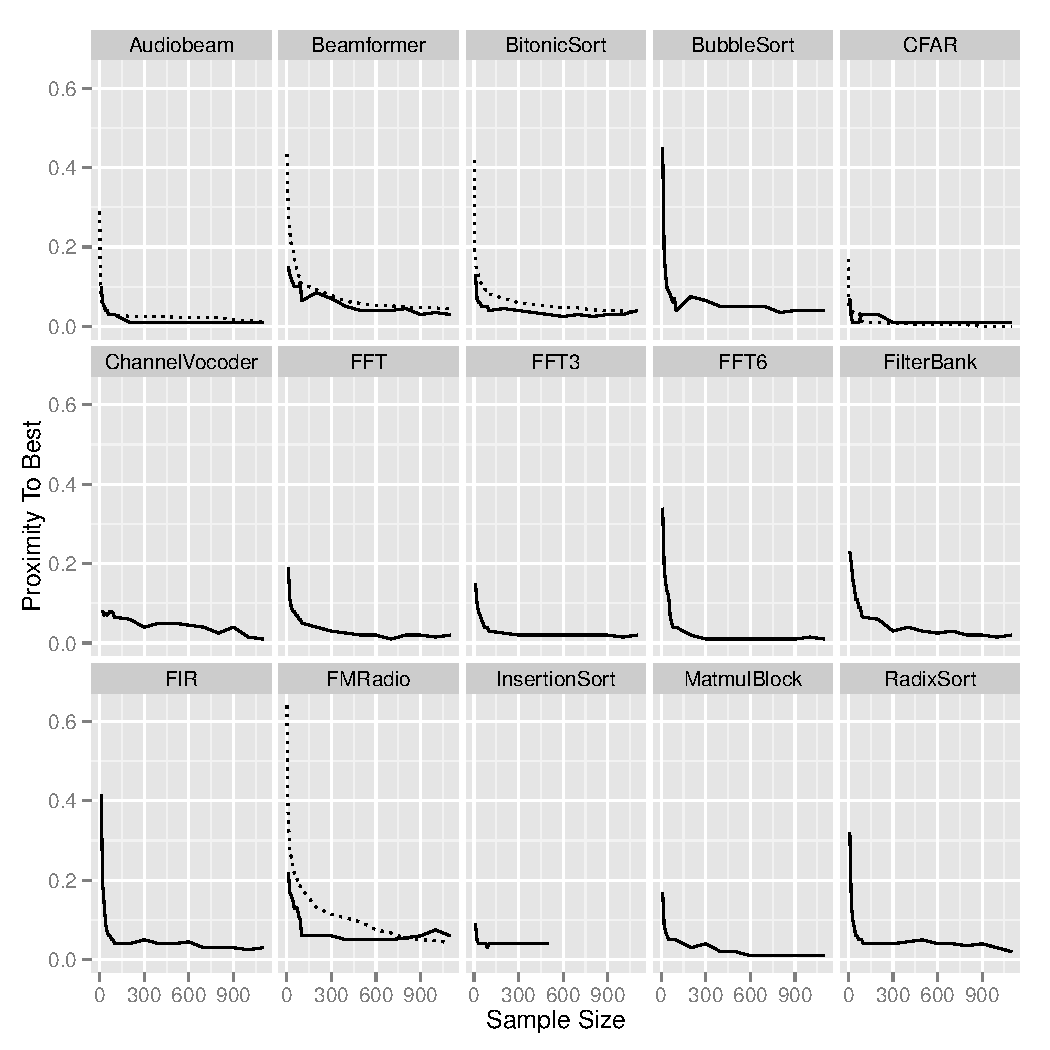
\includegraphics[width=1\textwidth]{streamit-paper/graphics/ESCProx.pdf}
    \caption{Statistical (plain line) and actual proximity (dotted line, this is only done for 5 benchmarks) to best performance using a subset of the sample space.}\label{fig:prox}
\end{figure}

%Define stopping criterion?
To gain confidence that the best configuration from the sample space is indeed close to the real best in the entire space, a statistical model based on the Early Stopping Criterion defined in~\cite{vuduc2003AutomaticPerf} is deployed.
This statistical model estimates, given a sample of the total space, if the best observed performance of that sample space is within a percentage of the statistical best performance, a more detailed explanation can be found in Chapter~\ref{chp:bg}.
The results demonstrate that the sample space selected is representative of the whole space.

Figure~\ref{fig:prox} shows, for each of the benchmarks, the proximity to the statistical best when increasing the sub-sample space given a maximal uncertainty of 5\%  (\ie minimum 95\% confidence).
As can be seen by the plain line, the model shows that the best sample point is actually within 5\% (0.05 proximity) of the best for all the benchmark.
The proximity is measured by taking the best currently observed point and comparing it to the latest discovered point.
To further prove that the statistical model based on the Stopping Criterion is indeed accurate, an exhaustive exploration of five benchmarks is conducted.
The dotted line in figure~\ref{fig:prox} shows the actual proximity to the best for \bench{Audiobeam}, \bench{Beamformer}, \bench{BitonicSort}, \bench{CFAR} and \bench{FMRadio}.
As can be seen after 1316 samples, the achieved performance is actually very similar to the one predicted by the statistical model, hence confirming prior work~\cite{vuduc2003AutomaticPerf}.
To summarize, it can be concluded that the best point found in the sample space of 1,316 points is at least within 5\% of the real best in the exhaustive space with 95\% confidence.

\subsection{Synthetic Benchmarks}

\begin{table}[t]
% The FFT need are variable
  \small
 \begin{tabular} { | l | l | l | }
 \hline
 & Av. Number of SplitJoins & Average Number of Filter Instances \\ \hline
 Selected Benchmarks & 14 & 52 \\ \hline 
 Synthetic & 22 & 64 \\ \hline
 \end{tabular}
 \caption{Data on the synthetic benchmarks compared to the selected benchmarks}~\label{tab:synthvsreal}
 \end{table}

One of the difficulties of building a machine learning based model for StreamIt is the lack of benchmarks available~\cite{wang2013partitionstreamit}.
To overcome this problem generating synthetic benchmarks can be a solution~\cite{cumminsopencl2017}.
Thus synthetic StreamIt benchmarks are generated and statistics are gathered from them in a similar style as in~\cite{wang2013partitionstreamit}.
In this chapter, the synthetic benchmarks are used to build a model for predicting the number of threads, which will be described later in section~\ref{sec:ml}

%Cite repository
To ensure that the synthetic benchmarks are representative of realistic benchmarks they are created using filters from a set of example StreamIt programs found in the example directory in the repository.
30 different possible filters with different incoming and outgoing rates and different inputs and outputs types are used to increase the variety of the dataset.
To ensure that the synthetic benchmarks are similar to real benchmarks, the total number of filters and split joins are within the average of the realistic benchmarks.

Table~\ref{tab:synthvsreal} gives the average number of SplitJoins and filter instances for the synthetic benchmarks vs the real benchmarks used in this chapter.
As can be seen, the synthetic benchmarks, on average, have more SplitJoins than the real benchmarks; this is due to the fact that a few of the benchmarks presented in the chapter don't have SplitJoins at all which can quickly reduce the average.
%Maybe say a bit more here.
Since these benchmarks are built to be used for predicting the number of threads an application should use, and SplitJoins are explicit declarations of task-level parallelism, having a higher average number of SplitJoins is not detrimental to building the model.
